% =====================================================================
% Informe Técnico — Taller de Proyecto Final
% Diplomatura en Inteligencia Artificial — UBA · FIUBA
% Track A: RAG / Chatbot
% Proyecto: Chatbot RAG para Movilidad Eléctrica CORADIR
% Autor: Carlos Salini
%
% Compilar en Overleaf con pdfLaTeX (carpeta autocontenida:
% este .tex + figs/). No requiere paquetes fuera de TeX Live estándar.
% =====================================================================
\documentclass[11pt,a4paper]{article}

\usepackage[utf8]{inputenc}
\usepackage[T1]{fontenc}
\usepackage[spanish,es-noshorthands]{babel}
\usepackage[margin=2.5cm]{geometry}
\usepackage{graphicx}
\usepackage{booktabs}
\usepackage{array}
\usepackage{float}
\usepackage{caption}
\usepackage{microtype}
\usepackage{enumitem}
\usepackage[hidelinks]{hyperref}
\usepackage{xcolor}

\graphicspath{{figs/}}
\captionsetup{font=small,labelfont=bf}
\setlist{nosep}

\newcommand{\code}[1]{\texttt{#1}}

\title{}
\date{}

\begin{document}

% ---------------------------------------------------------------------
% Carátula
% ---------------------------------------------------------------------
\begin{titlepage}
    \centering
    \vspace*{2cm}
    {\Large Universidad de Buenos Aires --- Facultad de Ingeniería\par}
    \vspace{0.3cm}
    {\large Diplomatura en Inteligencia Artificial\par}
    {\large Taller de Proyecto Final\par}
    \vspace{2.5cm}
    {\Huge\bfseries Chatbot RAG para Movilidad Eléctrica CORADIR\par}
    \vspace{0.6cm}
    {\Large Recuperación híbrida y respuesta extractiva sobre una base de
    conocimiento corporativa de vehículos eléctricos\par}
    \vspace{2.5cm}
    \begin{tabular}{rl}
        \textbf{Integrante:} & Carlos Salini \\[0.2cm]
        \textbf{Track:} & A --- RAG / Chatbot \\[0.2cm]
        \textbf{Fecha:} & 19/06/2026 \\[0.2cm]
        \textbf{Repositorio:} & \url{https://github.com/xKaruXx/DIIA-salini} \\
    \end{tabular}
    \vfill
\end{titlepage}

\tableofcontents
\newpage

% ---------------------------------------------------------------------
\section{Resumen Ejecutivo}
% ---------------------------------------------------------------------

CORADIR S.A. mantiene la información comercial y técnica de su línea de
vehículos eléctricos (modelos TITO, TITA, BARRE-TITA, CHIKI y la aplicación
CONTACTITO) en un documento JSON administrativo: especificaciones, precios,
agencias oficiales por provincia, infraestructura de carga y preguntas
frecuentes. Esa información no era consultable en lenguaje natural: el
personal de ventas y los visitantes del sitio web dependían de búsquedas
manuales sobre un documento jerárquico, sin trazabilidad de qué fuente
respalda cada dato.

Este proyecto implementa un chatbot web de tipo RAG (\emph{Retrieval
Augmented Generation}) que convierte esa base de conocimiento en un corpus
recuperable, medible y trazable. El sistema combina recuperación léxica y
vectorial (Chroma) sobre 111 documentos atómicos con \code{source\_path}
trazable, una capa de respuesta extractiva con términos de foco por tipo de
pregunta, y generación con un LLM local (\code{qwen3.5} servido por Ollama)
como ruta de respaldo, con guardrails de dominio. Todo el stack corre en
hardware local, sin servicios pagos.

Los resultados sobre el conjunto de evaluación de 64 casos con fuentes
esperadas fueron: exactitud por palabras clave de 64/64 (100\,\%) frente a un
baseline de 35/64 (54{,}7\,\%) antes de la mejora extractiva; Recall@5 de
retrieval de 0{,}969 con MRR de 0{,}916 y Top-1 de 0{,}875;
\emph{Context Faithfulness} medio de 0{,}895 en generación. La latencia de la
ruta extractiva es de 0{,}01\,s por consulta; la ruta generativa promedia
3{,}8\,s con el modelo recomendado (\code{qwen3.5:4b}) y el costo marginal por
consulta es nulo por tratarse de modelos locales.

La conclusión principal es que, en este corpus, el cuello de botella no
estaba en el retrieval sino en la selección del fragmento correcto dentro del
documento recuperado: 24 de los 29 fallos del baseline ya tenían la fuente
esperada en el top-5. La principal limitación es que el conjunto de
evaluación se usó iterativamente durante la mejora, por lo que el 100\,\%
final indica cobertura del benchmark y no una garantía de exactitud ante
consultas reales nuevas; la validación con muestras no vistas queda como
trabajo futuro inmediato.

% ---------------------------------------------------------------------
\section{Justificación de la Solución}
% ---------------------------------------------------------------------

\subsection{Contexto y problema}

CORADIR es un fabricante argentino de vehículos eléctricos con una red de
agencias en varias provincias. Su información de productos cambia con
frecuencia (precios en USD, disponibilidad, accesorios, condiciones de
compra) y se administra en un JSON jerárquico de uso interno
(\code{dataset/dataset\_movilidad.json}). Las consultas típicas que recibe la
empresa --- ``¿cuánta autonomía tiene el TITO S5?'', ``¿qué agencia hay en
Moreno?'', ``¿el precio incluye patentamiento?'' --- requieren conocer la
estructura del documento para responderlas, y no existía forma de auditar de
dónde salió cada respuesta.

El problema técnico es entonces doble: (i) hacer recuperable en lenguaje
natural una base de conocimiento administrativa con datos exactos (precios,
direcciones, especificaciones), donde una respuesta aproximada es peor que no
responder; y (ii) hacerlo de forma medible y trazable, de modo que cada
respuesta pueda rastrearse hasta el campo del JSON que la respalda. El
requisito de datos exactos condiciona todo el diseño: el sistema prioriza
extraer literalmente el dato de la fuente recuperada antes que parafrasearlo
con un modelo generativo.

\subsection{Decisiones de diseño}

Cada decisión se documenta con el esquema decisión $\rightarrow$ alternativas
$\rightarrow$ criterio $\rightarrow$ trade-off asumido. La
Tabla~\ref{tab:decisiones} resume las seis decisiones principales; las
subsecciones siguientes desarrollan las menos evidentes.

\begin{table}[H]
\centering
\small
\begin{tabular}{p{3.4cm}p{3.6cm}p{3.6cm}p{3.6cm}}
\toprule
\textbf{Decisión} & \textbf{Alternativas} & \textbf{Criterio} & \textbf{Trade-off asumido} \\
\midrule
Documentos atómicos por campo del JSON (media 44 tokens) &
Chunking clásico por tamaño fijo (200--400 tokens) con solapamiento &
Los datos son campos puntuales; el EDA mostró mediana de 24 tokens
(§\ref{sec:eda}) &
111 docs muy cortos $\Rightarrow$ Precision@5 baja por chunks ``extra''
recuperados \\
\addlinespace
Retrieval híbrido: léxico + vectorial &
Solo vectorial; solo léxico (BM25-like) &
Recall@5 y Top-1 sobre 64 casos con fuentes esperadas &
Dos índices a mantener; ranking léxico sensible a stopwords \\
\addlinespace
Embeddings \code{nomic-embed-text-v2-moe} &
\code{nomic-embed-text}, \code{embeddinggemma}, \code{qwen3-embedding:0.6b} &
Matriz de retrieval vectorial puro sobre 64 casos
(Tabla~\ref{tab:embeddings}) &
No es el mejor en MRR (lo supera \code{embeddinggemma}); cambio diferido \\
\addlinespace
LLM \code{qwen3.5:4b} para la demo &
11 modelos locales de 270M a 32B evaluados &
Score sintético + latencia + peso en disco (Fig.~\ref{fig:tradeoff}) &
4{,}19/5 vs.\ 4{,}29/5 del \code{qwen3.5:latest}, a cambio de
$-26\,\%$ de latencia y la mitad de memoria \\
\addlinespace
Mejorar la capa extractiva antes que cambiar embeddings &
Reindexar con otro embedding; reranking con cross-encoder &
24/29 fallos ya tenían la fuente en top-5: el problema era la selección de
líneas &
La capa extractiva agrega reglas específicas del dominio que hay que
mantener \\
\addlinespace
Stack 100\,\% local (Ollama + Chroma + SQLite) &
APIs pagas (OpenAI) para LLM y embeddings &
Costo por consulta, privacidad de datos comerciales, reproducibilidad
sin claves &
Modelos locales más débiles que los de frontera; latencia ligada al
hardware \\
\bottomrule
\end{tabular}
\caption{Resumen de decisiones de diseño con alternativas, criterio y costo asumido.}
\label{tab:decisiones}
\end{table}

\subsubsection{Documentos atómicos en lugar de chunking por tamaño}

El corpus no es texto corrido sino un árbol de campos cortos (precio de un
modelo, dirección de una agencia, una pregunta frecuente). Se comparó
conceptualmente contra el chunking clásico de 200--400 tokens con
solapamiento visto en clase: agrupar campos heterogéneos en un mismo chunk
hubiera mezclado, por ejemplo, precios de dos modelos distintos en un mismo
fragmento, aumentando el riesgo de que el LLM tome el dato equivocado. Se
optó por generar un documento por campo u objeto del JSON
(\code{scripts/prepare\_dataset.py}), cada uno con metadatos
\code{\{id, section, title, source\_path\}}. El costo es un corpus de
documentos muy cortos que penaliza la Precision@5 (se recuperan vecinos
``extra''), aceptado porque Recall y Top-1 son las métricas que condicionan
la respuesta final.

\subsubsection{Por qué no se cambió el modelo de embeddings al final}\label{sec:noembed}

La evaluación de embeddings (§\ref{sec:embeddings}) mostró que
\code{embeddinggemma} y \code{qwen3-embedding:0.6b} superan a
\code{nomic-embed-text-v2-moe} en retrieval vectorial puro. Sin embargo, el
análisis de fallos del benchmark extendido mostró que 24 de los 29 casos
fallidos ya recuperaban la fuente correcta en el top-5: cambiar el embedding
atacaba el 17\,\% del problema (5 fallos de retrieval) y la mejora extractiva
el 83\,\% restante. Se priorizó la capa extractiva, que llevó el resultado a
64/64 sin reindexar. Reevaluar el embedding quedó como trabajo futuro: es una
decisión de secuenciamiento, no un descarte.

\subsubsection{Por qué no hay reranking con cross-encoder}

Se consideró agregar un reranker neuronal sobre el top-K recuperado. Se
descartó por dos razones medidas en el propio sistema: (i) el primer
documento relevante ya aparece en promedio en la posición 1{,}22 del ranking
híbrido (§\ref{sec:retrieval}), de modo que el margen de mejora de
reordenar es chico; y (ii) el patrón de fallos no era de orden sino de
extracción del campo dentro del documento. El costo evitado es la latencia y
memoria de un segundo modelo en una máquina que ya sirve el LLM y los
embeddings.

% ---------------------------------------------------------------------
\section{EDA y Descubrimientos}\label{sec:eda}
% ---------------------------------------------------------------------

\subsection{Descripción del corpus}

La fuente es \code{dataset/dataset\_movilidad.json} (47\,KB), el documento
administrativo real de CORADIR Movilidad Eléctrica: información
institucional, catálogo de vehículos con especificaciones, precios por
variante, agencias por provincia, infraestructura de carga (Ecocarga),
preguntas frecuentes y condiciones comerciales. El preprocesamiento lo
convierte en \code{dataset/knowledge\_base\_movilidad.jsonl}. La
Tabla~\ref{tab:corpus} resume las métricas del EDA, calculadas con los
criterios de riqueza léxica del material de clase (TTR y MATTR con ventana
50)~\cite{covington}.

\begin{table}[H]
\centering
\begin{tabular}{lr}
\toprule
\textbf{Métrica} & \textbf{Valor} \\
\midrule
Documentos indexables & 111 \\
Tokens totales & 4\,907 \\
Tokens por documento (media / mediana / p90 / máx.) & 44{,}21 / 24 / 105 / 401 \\
TTR promedio & 0{,}834 \\
MATTR promedio (ventana 50) & 0{,}854 \\
Documentos muy cortos ($<$ 30 tokens) & 67 \\
Documentos muy largos ($>$ 200 tokens) & 2 \\
Documentos con baja densidad léxica & 0 \\
\bottomrule
\end{tabular}
\caption{Métricas del EDA sobre el corpus preprocesado (111 documentos).}
\label{tab:corpus}
\end{table}

\subsection{Hallazgos y decisiones derivadas}

\paragraph{Hallazgo 1: el corpus es de documentos muy cortos y asimétricos.}
La distribución de longitudes (Figura~\ref{fig:tokens}) está fuertemente
sesgada: mediana de 24 tokens, con 67 documentos por debajo de 30 tokens y
solo 2 outliers largos (la ficha técnica completa del TITO, 401 tokens, y el
listado de agencias de Buenos Aires, 388 tokens). \emph{...y por eso
decidimos} no aplicar chunking por tamaño: fragmentar documentos que en su
mayoría ya son atómicos solo podía romper unidades de significado. Los dos
documentos largos se trataron en la capa extractiva (selección de líneas
dentro del documento) en lugar de subdividirlos en el índice.

\begin{figure}[H]
    \centering
    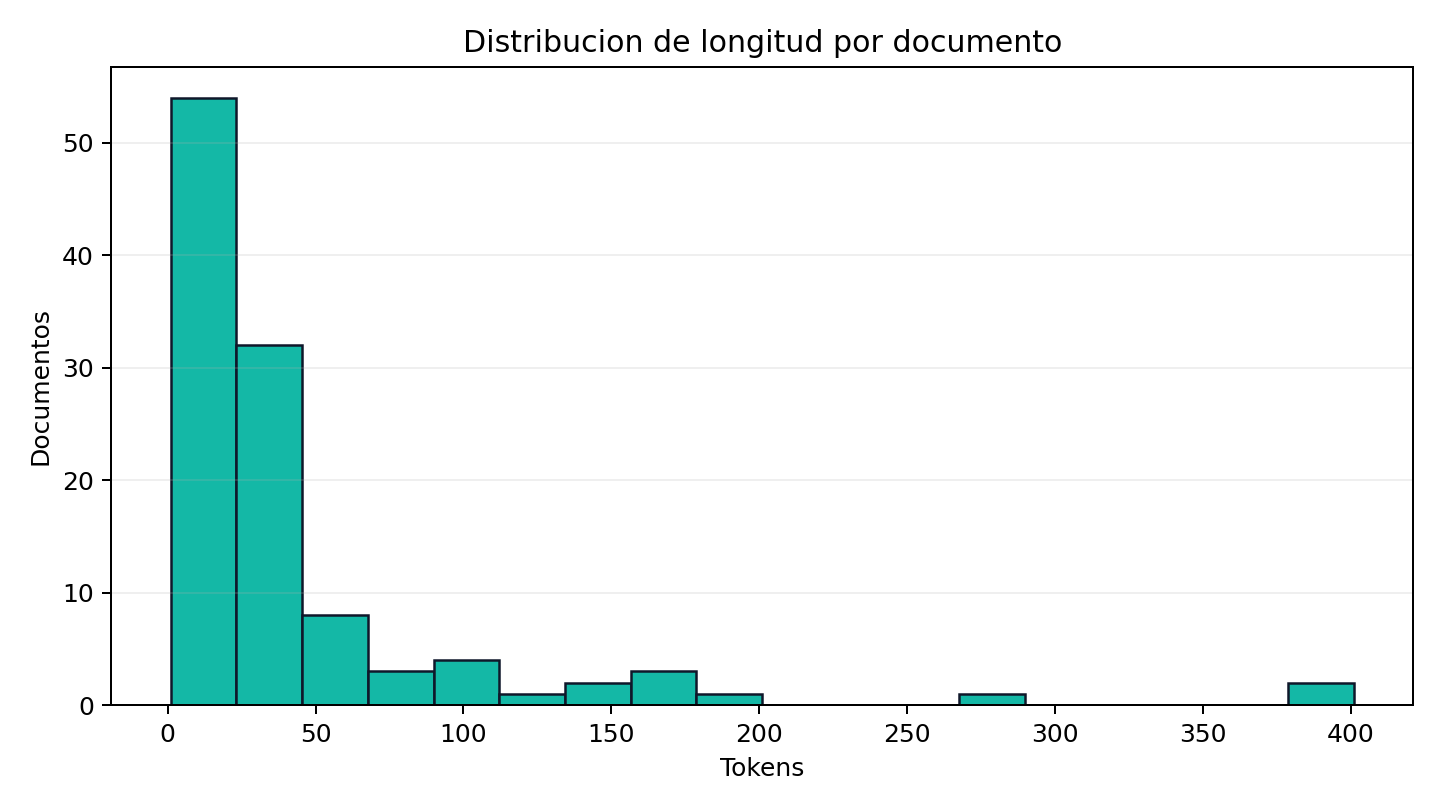
\includegraphics[width=0.82\textwidth]{corpus_token_distribution.png}
    \caption{Distribución de longitud por documento del corpus (tokens). La
    masa se concentra debajo de 50 tokens, con dos outliers (388 y 401
    tokens) que corresponden a la ficha técnica del TITO y a las agencias de
    Buenos Aires.}
    \label{fig:tokens}
\end{figure}

\paragraph{Hallazgo 2: la estructura jerárquica del JSON es un activo de
trazabilidad.} Cada campo del JSON tiene una ruta natural
(p.\,ej.\ \code{vehiculos\_detalles.TITO.modelos\_disponibles[1]}).
\emph{...y por eso decidimos} conservar esa ruta como metadato
\code{source\_path} de cada documento, lo que después habilitó definir
\code{expected\_sources} por caso de evaluación y auditar el retrieval contra
fuentes esperadas (§\ref{sec:retrieval}), además de poder mostrar el
respaldo de cada respuesta.

\paragraph{Hallazgo 3: la riqueza léxica no justificaba normalización
agresiva.} Con MATTR promedio de 0{,}854 y ningún documento con baja densidad
léxica, no había evidencia de vocabulario degenerado o repetitivo.
\emph{...y por eso decidimos} no aplicar lematización ni stemming global
sobre el corpus, y concentrar el esfuerzo de normalización solo en la
búsqueda léxica (minúsculas, acentos y stopwords interrogativas), preservando
los valores literales --- ``USD 17.731,25'', ``Ficha 2073'' --- que el usuario
necesita recibir exactos.

\paragraph{Hallazgo 4: la distribución por sección es desbalanceada.}
El corpus concentra documentos en \code{vehiculos\_detalles}, \code{precios}
y \code{agencias} (Figura~\ref{fig:secciones}), que coinciden con las
categorías de consulta más frecuentes. \emph{...y por eso decidimos} diseñar
el conjunto de evaluación extendido respetando esa proporción (22 casos de
vehículos y 12 de precios sobre 64) y ponderar en la búsqueda léxica las
entidades de dominio (TITO, TITA S2, CHIKI, CONTACTITO Plus, Ecocarga) por
sobre términos genéricos.

\begin{figure}[H]
    \centering
    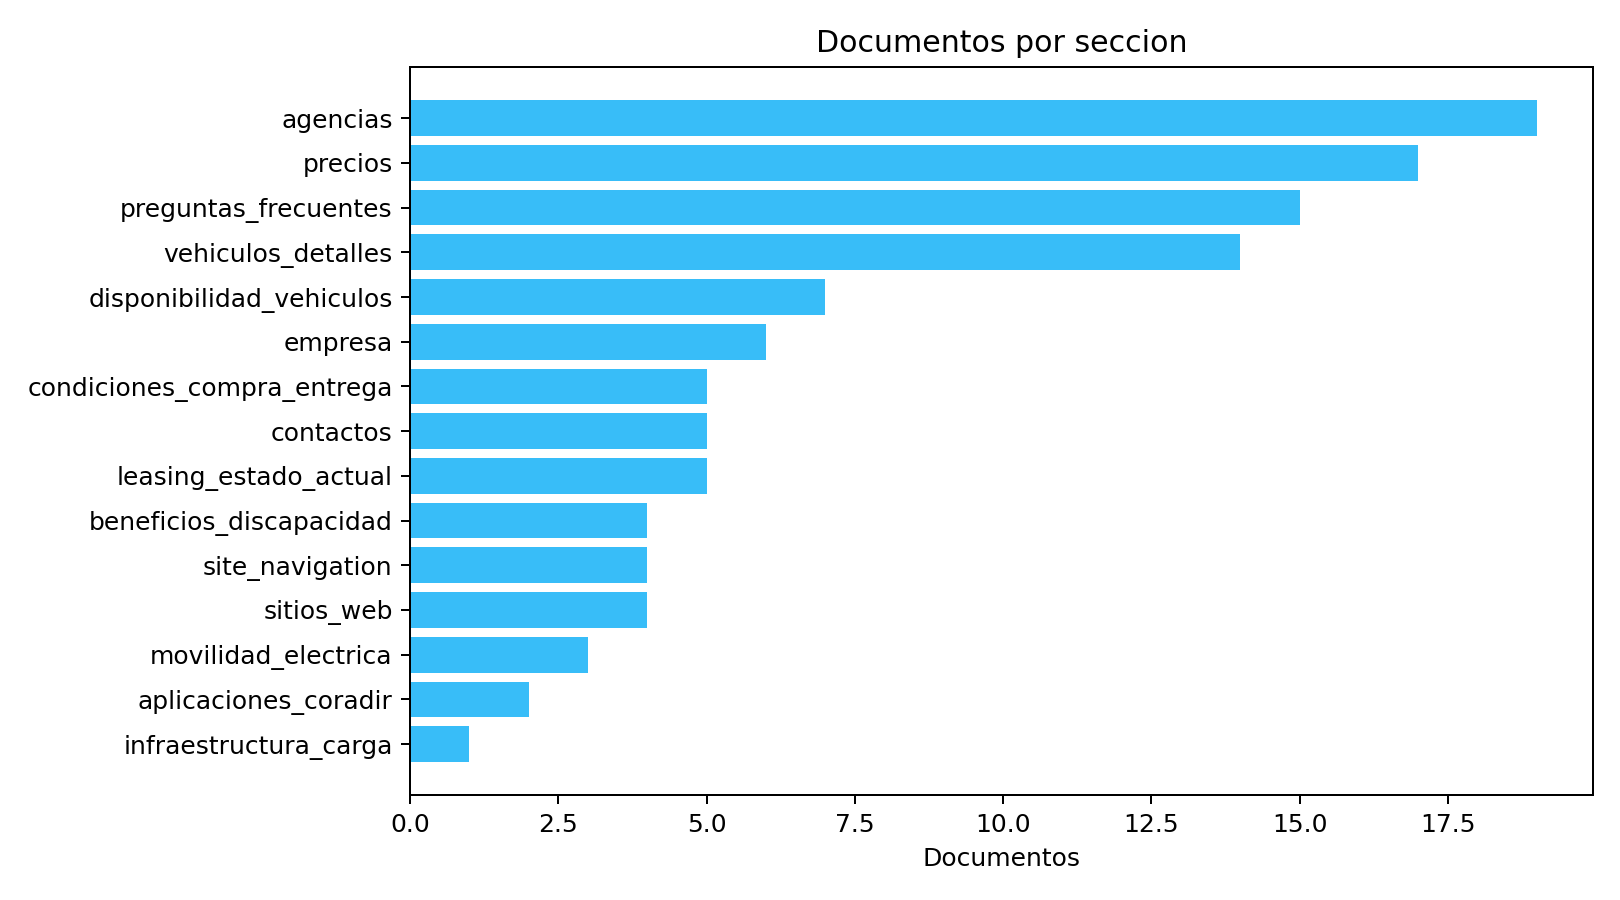
\includegraphics[width=0.82\textwidth]{corpus_documents_by_section.png}
    \caption{Documentos por sección del corpus. El desbalance guio la
    composición del conjunto de evaluación y la ponderación de entidades en
    la búsqueda léxica.}
    \label{fig:secciones}
\end{figure}

Los documentos extremos detectados por el EDA (campos de 1--5 tokens como
\code{empresa.fundacion} o \code{sitios\_web.principal}) se revisaron
manualmente y se conservaron: contienen datos puntuales (URLs, fechas,
emails) que son justamente el tipo de dato exacto que el sistema debe poder
devolver.

% ---------------------------------------------------------------------
\section{Arquitectura Propuesta}
% ---------------------------------------------------------------------

\subsection{Visión general}

La Figura~\ref{fig:arquitectura} muestra el pipeline completo, separado en un
flujo \emph{offline} de ingesta e indexado y un flujo \emph{online} de
consulta. El diseño sigue el patrón general de RAG con índice precomputado
(\emph{retrieve-then-read}~\cite{lewis2020rag}), con dos particularidades:
una ruta extractiva que responde sin LLM cuando la búsqueda léxica encuentra
el dato exacto, y guardrails de dominio que cortan antes de recuperar.

\begin{figure}[H]
    \centering
    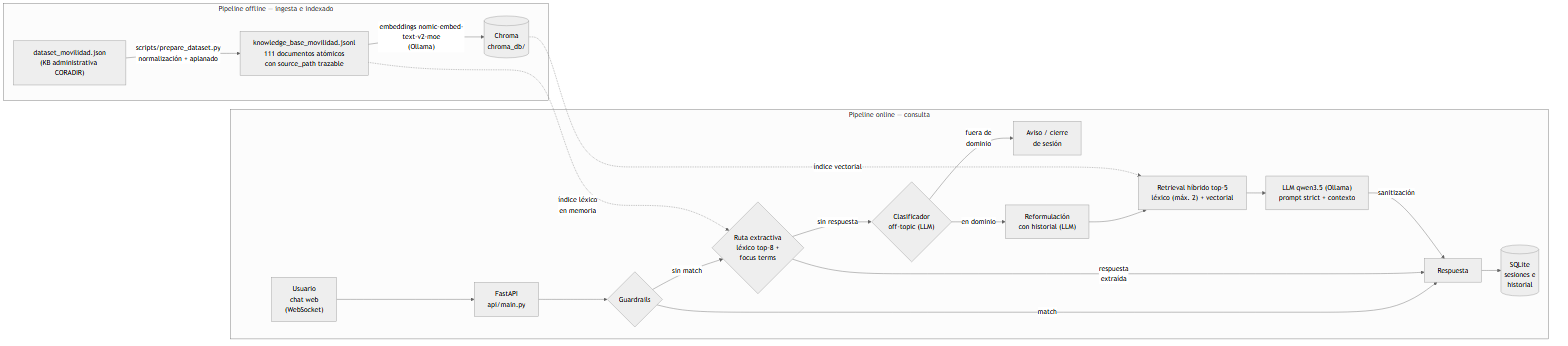
\includegraphics[width=\textwidth]{arquitectura_pipeline.png}
    \caption{Arquitectura del sistema. Flujo offline (ingesta e indexado) y
    flujo online (consulta) con sus artefactos: JSONL de 111 documentos,
    índice Chroma en \code{chroma\_db/}, e historial en SQLite. Figura de
    elaboración propia (fuente Mermaid en
    \code{docs/informe\_tecnico/arquitectura\_pipeline.mmd}).}
    \label{fig:arquitectura}
\end{figure}

\subsection{Etapas del pipeline}

Para cada etapa se declara entrada $\rightarrow$ proceso $\rightarrow$ salida
$\rightarrow$ almacenamiento.

\begin{description}[style=nextline]
    \item[Ingesta y preprocesamiento.] Entrada:
    \code{dataset/dataset\_movilidad.json} (JSON jerárquico administrativo).
    Proceso: \code{scripts/prepare\_dataset.py} normaliza encoding, aplana el
    árbol y genera un documento atómico por campo u objeto, conservando la
    ruta de origen. Salida: \code{\{id, section, title, content,
    source\_path\}} por línea. Almacenamiento:
    \code{dataset/knowledge\_base\_movilidad.jsonl} (111 documentos,
    versionado en el repositorio).

    \item[Vectorización e indexado.] Entrada: el JSONL anterior. Proceso:
    embeddings con \code{nomic-embed-text-v2-moe} (768 dimensiones) servidos
    por Ollama; creación o carga del índice al iniciar la API. Salida: índice
    vectorial persistente. Almacenamiento: \code{chroma\_db/} (Chroma
    0.6.3), una colección por modelo de embeddings para poder comparar
    configuraciones sin pisar índices.

    \item[Guardrails.] Entrada: la pregunta del usuario. Proceso: reglas
    previas al retrieval para casos sensibles (consultas de precios fuera de
    catálogo, pedidos de contacto, temas de seguridad) con respuestas
    controladas; límite de mensajes fuera de dominio por sesión con cierre
    automático. Salida: respuesta controlada o pase a la siguiente etapa.
    Almacenamiento: no aplica (reglas en \code{api/chat\_service.py}).

    \item[Ruta extractiva.] Entrada: pregunta en dominio. Proceso: búsqueda
    léxica sobre los 111 documentos (top-8) con normalización, remoción de
    stopwords interrogativas y ponderación de entidades; selección de líneas
    dentro del documento según \emph{términos de foco} por tipo de pregunta
    (colores, dimensiones, direcciones, costos no incluidos, etc.) con un
    presupuesto dinámico de líneas; expansión de bloques estructurados tipo
    lista. Salida: respuesta extractiva literal con su fuente, o vacío si no
    hay match suficiente. Almacenamiento: índice léxico en memoria,
    construido desde el JSONL al iniciar.

    \item[Recuperación híbrida (ruta generativa).] Entrada: pregunta
    reformulada con el historial de la sesión (un LLM reescribe la consulta
    si hay contexto conversacional previo). Proceso: combinación de
    resultados léxicos (máximo 2 fragmentos) y vectoriales de Chroma hasta
    top-5. Salida: contexto concatenado con títulos y fuentes.
    Almacenamiento: no persiste; se arma por consulta.

    \item[Generación y verificación.] Entrada: contexto recuperado +
    pregunta + historial. Proceso: prompt con variante \code{strict} (instruye
    responder solo con el contexto y admitir ``no se especifica'' cuando el
    dato no está), generación con \code{qwen3.5} vía Ollama, sanitización de
    la salida (remoción de trazas de razonamiento del modelo). Salida:
    respuesta final. Almacenamiento: mensajes y sesiones en SQLite
    (\code{chatbot\_movilidad.db}) vía SQLAlchemy.

    \item[Serving.] Entrada: mensajes del usuario desde el chat web. Proceso:
    FastAPI con WebSocket (\code{api/main.py}), autenticación JWT de sesión,
    rate limiting por IP para acciones de contacto, y webhooks opcionales a
    n8n para derivación comercial. Salida: respuesta en el chat embebido
    (\code{chat\_assets/}). Almacenamiento: SQLite local (PostgreSQL
    configurable vía \code{DATABASE\_URL}).
\end{description}

\subsection{Stack tecnológico}

La Tabla~\ref{tab:stack} resume los componentes con sus versiones y el rol
de cada uno en el pipeline.

\begin{table}[H]
\centering
\small
\begin{tabular}{llll}
\toprule
\textbf{Componente} & \textbf{Tecnología} & \textbf{Versión} & \textbf{Rol} \\
\midrule
API y serving & FastAPI + Uvicorn & 0.115.8 / 0.34.0 & HTTP, WebSocket del chat, JWT \\
Orquestación RAG & LangChain (+ community, ollama) & 0.3.19 & Prompts, memoria, cadenas \\
Vector store & Chroma & 0.6.3 & Índice vectorial persistente \\
Embeddings & \code{nomic-embed-text-v2-moe} & 475M par., 768d & Vectorización multilingüe \\
LLM (demo) & \code{qwen3.5:4b} vía Ollama & 4B par. & Generación ruta LLM \\
LLM (benchmark) & \code{qwen3.5:latest} vía Ollama & 32B par. & Generación en evaluaciones \\
Persistencia & SQLAlchemy + SQLite & 2.0.38 & Sesiones, mensajes, rate limit \\
Tokenización & tiktoken & 0.9.0 & Conteos de tokens del EDA \\
Análisis y gráficos & pandas + matplotlib & 2.2.3 / 3.10.0 & Benchmarks y figuras \\
Frontend & HTML/CSS/JS + WebSocket & --- & Chat web embebible \\
Integración externa & n8n (webhooks, opcional) & --- & Derivación de contactos \\
\bottomrule
\end{tabular}
\caption{Stack tecnológico con versiones (según \code{requirements.txt} y \code{.env}).}
\label{tab:stack}
\end{table}

Criterio de reproducibilidad: con el repositorio, \code{requirements.txt},
\code{.env.example} y los comandos del Anexo~\ref{anexo:comandos}, otro
equipo puede regenerar el JSONL, reindexar y repetir todos los benchmarks de
la Sección~\ref{sec:evaluacion}; los resultados citados están versionados
como JSON en \code{docs/}.

% ---------------------------------------------------------------------
\section{Evaluación de Resultados}\label{sec:evaluacion}
% ---------------------------------------------------------------------

\subsection{Protocolo de evaluación}

Se construyeron tres conjuntos de evaluación versionados en
\code{dataset/}:

\begin{itemize}
    \item \textbf{MVP} (15 casos): preguntas factuales directas con
    \code{expected\_keywords}; sirvió como prueba de humo del MVP.
    \item \textbf{Extendido} (64 casos): cubre 13 categorías (vehículos,
    precios, agencias, carga, compra, empresa, etc.) respetando la
    distribución del corpus. Cada caso define \code{expected\_keywords} (el
    dato exacto que debe aparecer en la respuesta) y
    \code{expected\_sources} (los \code{source\_path} que la respaldan), lo
    que permite evaluar por separado la respuesta final y el retrieval.
    \item \textbf{Matriz manual de modelos} (21 preguntas $\times$ 11
    modelos): 7 factuales, 7 ambiguas y 7 fuera de dominio, para seleccionar
    el LLM de chat.
\end{itemize}

El criterio de acierto del benchmark automatizado es estricto: un caso pasa
solo si la respuesta contiene todas las \code{expected\_keywords} (valores
literales como ``17.731,25'' o ``ISO 9001''). No hay split train/test en el
sentido clásico porque no se entrena ningún modelo; el riesgo análogo ---
sobreajuste de las reglas extractivas al conjunto de evaluación --- existe y
se discute como limitación en §\ref{sec:limitaciones}. El ground truth de
\code{expected\_sources} se construyó manualmente revisando el JSON original.

\subsection{Resultados comparativos}

La Tabla~\ref{tab:comparativa} muestra la progresión completa, del baseline a
la versión final, sobre los mismos 64 casos y con la misma configuración de
retrieval (híbrido, top-5, \code{qwen3.5:latest} +
\code{nomic-embed-text-v2-moe}). El baseline obligatorio es el sistema RAG
``ingenuo'': recuperación más generación, sin la capa extractiva mejorada.

\begin{table}[H]
\centering
\begin{tabular}{lrrl}
\toprule
\textbf{Configuración} & \textbf{Casos correctos} & \textbf{Accuracy} & \textbf{Cambio introducido} \\
\midrule
MVP (15 casos, humo) & 15/15 & 100{,}0\,\% & --- \\
\midrule
Baseline extendido & 35/64 & 54{,}7\,\% & RAG sin extracción mejorada \\
Iteración 1 & 46/64 & 71{,}9\,\% & Extracción por bloques estructurados \\
Iteración 2 & 57/64 & 89{,}1\,\% & Ranking por entidad + stopwords \\
\textbf{Sistema final (it.\ 3)} & \textbf{64/64} & \textbf{100{,}0\,\%} & Ajustes de casos restantes \\
\bottomrule
\end{tabular}
\caption{Tabla comparativa de configuraciones sobre el benchmark extendido de
64 casos (fuente: \code{docs/benchmark\_extendido\_strict\_*.json}). La
iteración 1 introdujo 2 regresiones que se documentan en
§\ref{sec:errores} y quedaron corregidas en la iteración 3.}
\label{tab:comparativa}
\end{table}

El salto de 54{,}7\,\% a 100\,\% se logró sin cambiar el corpus, el índice ni
el modelo de embeddings: aísla el efecto de la capa extractiva. La lectura
honesta de la última fila exige dos aclaraciones: (i) el conjunto de
evaluación se usó para diagnosticar y corregir entre iteraciones, así que
mide cobertura del benchmark, no generalización; y (ii) el criterio por
keywords no evalúa fluidez ni utilidad percibida, solo presencia del dato
exacto.

\subsection{Métricas de retrieval}\label{sec:retrieval}

Sobre la corrida final se auditaron los 257 chunks recuperados en los 64
casos contra las fuentes esperadas (Tabla~\ref{tab:retrieval}).

\begin{table}[H]
\centering
\begin{tabular}{lr}
\toprule
\textbf{Métrica (top-5, retrieval híbrido)} & \textbf{Valor} \\
\midrule
Recall@5 (medio) & 0{,}969 \\
Precision@5 (media) & 0{,}319 \\
MRR & 0{,}916 \\
Top-1 source accuracy & 0{,}875 \\
Posición media del primer chunk relevante & 1{,}22 \\
Casos con alguna fuente esperada en top-5 & 63/64 \\
Casos con \emph{todas} las fuentes esperadas en top-5 & 61/64 \\
\bottomrule
\end{tabular}
\caption{Auditoría de retrieval sobre la corrida final
(\code{docs/auditoria\_rag\_chunks\_clase6.json}).}
\label{tab:retrieval}
\end{table}

La combinación Recall@5 alto (0{,}969) con Precision@5 baja (0{,}319) es una
consecuencia directa de la decisión de corpus atómico: casi siempre la fuente
correcta está entre los 5 recuperados (y en promedio en la posición 1{,}22),
pero la acompañan vecinos cortos de la misma sección. El diagnóstico
automático de la auditoría clasificó 46 de 64 casos como ``revisar chunks
extra'' y solo 3 como ``fuente esperada ausente'', lo que confirma que el
ruido --- y no la falta de cobertura --- es el costo a vigilar.

\subsection{Métricas de generación}

Con la metodología de la clase 6 se midieron \emph{Token Overlap} (presencia
de las keywords esperadas en la respuesta) y \emph{Context Faithfulness}
(proporción de la respuesta respaldada por el contexto recuperado) sobre los
64 casos: Token Overlap medio de 1{,}0 y Context Faithfulness medio de
0{,}895, con 51/64 casos por encima del umbral de 0{,}8. Los 13 casos
restantes quedaron marcados como ``posible alucinación o contexto no
trazado''; la inspección mostró que se concentran en categorías con
documentos muy cortos (contacto: 0{,}267; sitios web: 0{,}429), donde la
respuesta extractiva agrega texto de encabezado que la métrica no encuentra
en el chunk auditado. Es un límite de la métrica y del trazado, no
necesariamente una alucinación: distinguirlos requiere la revisión manual
que se propone como trabajo futuro.

\subsection{Selección del modelo de embeddings}\label{sec:embeddings}

Se evaluaron los cuatro embeddings disponibles localmente en modo vectorial
puro (sin búsqueda léxica ni generación), para medir el componente semántico
aislado sobre los mismos 64 casos (Tabla~\ref{tab:embeddings}).

\begin{table}[H]
\centering
\begin{tabular}{lrrrr}
\toprule
\textbf{Embedding} & \textbf{Precision@5} & \textbf{Recall@5} & \textbf{MRR} & \textbf{Top-1} \\
\midrule
\code{embeddinggemma} (307M) & 24{,}4\,\% & 80{,}5\,\% & \textbf{69{,}5\,\%} & \textbf{60{,}9\,\%} \\
\code{qwen3-embedding:0.6b} (596M) & 24{,}1\,\% & \textbf{81{,}2\,\%} & 67{,}9\,\% & 57{,}8\,\% \\
\code{nomic-embed-text-v2-moe} (475M) & 20{,}0\,\% & 74{,}2\,\% & 64{,}3\,\% & 54{,}7\,\% \\
\code{nomic-embed-text} (137M) & 13{,}4\,\% & 43{,}8\,\% & 29{,}9\,\% & 20{,}3\,\% \\
\bottomrule
\end{tabular}
\caption{Retrieval vectorial puro por modelo de embeddings, top-5, 64 casos
(\code{docs/evaluacion\_embeddings\_locales.md}).}
\label{tab:embeddings}
\end{table}

Dos conclusiones salieron de esta matriz. Primero, el embedding inicial
(\code{nomic-embed-text}) era el eslabón más débil del sistema: con 43{,}8\,\%
de Recall@5 vectorial, la cobertura del baseline dependía de la búsqueda
léxica. Se migró a \code{nomic-embed-text-v2-moe}, que casi duplica el
Recall@5 vectorial. Segundo, \code{embeddinggemma} y
\code{qwen3-embedding:0.6b} son mejores aún en modo vectorial puro; no se
adoptaron en esta versión porque la mejora extractiva ya había llevado el
benchmark a 64/64 con el índice existente (decisión de secuenciamiento
justificada en §\ref{sec:noembed}), y quedan como candidatos medidos para la próxima
iteración.

\subsection{Selección del LLM de chat}

Sobre la matriz manual (21 preguntas $\times$ 11 modelos locales, 231
respuestas) se midió un score sintético de calidad 1--5 por respuesta,
separando preguntas factuales, ambiguas y fuera de dominio, junto con la
latencia promedio y el peso local del modelo (Figura~\ref{fig:tradeoff}).
Los mejores fueron \code{qwen3.5:latest} (score 4{,}29; 16/21 respuestas
aceptables; 5{,}18\,s; 6{,}6\,GB) y \code{qwen3.5:4b} (4{,}19; 15/21;
3{,}84\,s; 3{,}4\,GB). Se eligió \code{qwen3.5:4b} como modelo de la demo:
cede 0{,}10 de score y una respuesta aceptable a cambio de 26\,\% menos
latencia y la mitad de memoria, lo que permite convivir con los embeddings en
la misma GPU/CPU. Modelos menores quedaron descartados con evidencia:
\code{gemma3:270m} produjo respuestas vacías (8/21) y
\code{lfm2.5-thinking:1.2b} no emitió respuesta final utilizable en ningún
caso (solo traza de razonamiento). \code{nemotron-3-nano:4b} destacó en
rechazar preguntas fuera de dominio (5{,}0/5) y se anotó como alternativa si
se prioriza ese comportamiento.

\begin{figure}[H]
    \centering
    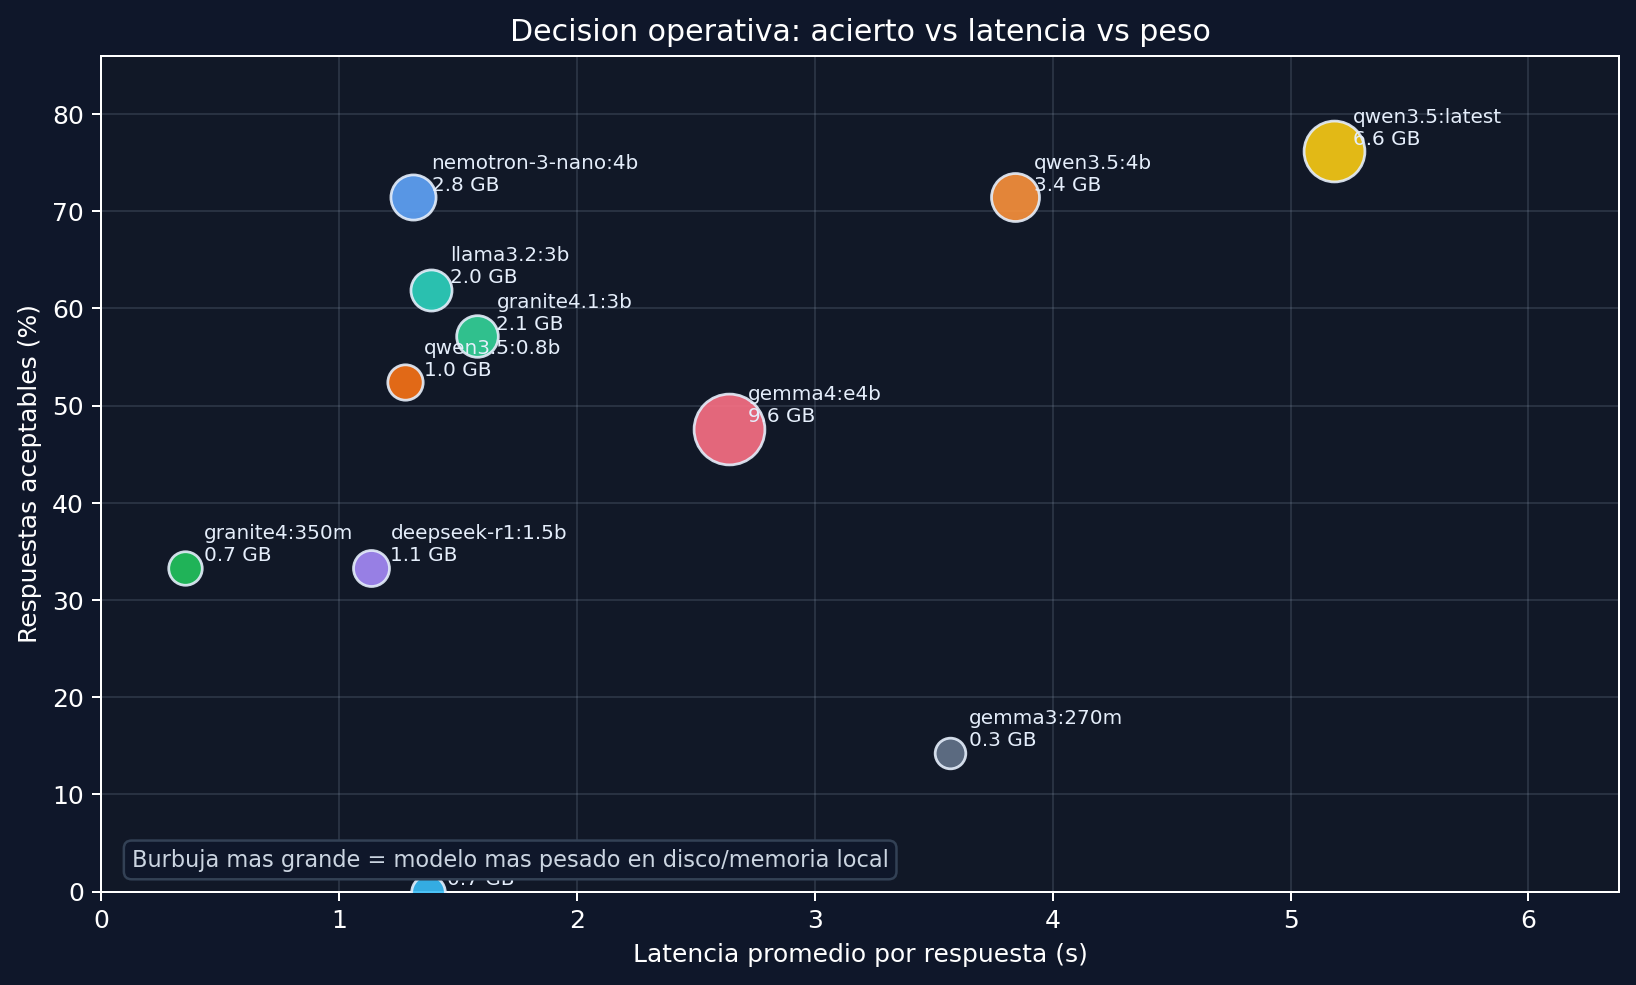
\includegraphics[width=0.9\textwidth]{manual_model_tradeoff.png}
    \caption{Decisión operativa de LLM: porcentaje de respuestas aceptables
    vs.\ latencia promedio; el tamaño de burbuja es el peso local del modelo.
    \code{qwen3.5:4b} es el compromiso elegido para la demo.}
    \label{fig:tradeoff}
\end{figure}

\subsection{Métricas operativas}

\begin{itemize}
    \item \textbf{Latencia.} La ruta extractiva responde en 0{,}01\,s
    promedio (benchmark de 64 casos). La ruta generativa depende del modelo:
    3{,}84\,s promedio con \code{qwen3.5:4b} y 5{,}18\,s con
    \code{qwen3.5:latest} (matriz manual). En operación, la mayoría de las
    preguntas factuales del dominio resuelven por la ruta extractiva.
    \item \textbf{Costo.} Nulo por consulta: todos los modelos corren
    localmente vía Ollama. El costo real es fijo (hardware y energía), con
    requisito de $\sim$3{,}4\,GB de disco/memoria para el LLM de demo más
    $\sim$1\,GB del embedding.
    \item \textbf{Huella del índice.} 111 documentos $\times$ 768 dimensiones:
    el índice Chroma es de tamaño despreciable y se reconstruye en segundos,
    lo que permitió iterar configuraciones de embeddings sin fricción.
\end{itemize}

\subsection{Análisis de errores}\label{sec:errores}

Se documentan cuatro fallas reales observadas durante el desarrollo, con su
causa raíz y corrección. Las dos primeras provienen del baseline extendido;
las dos últimas son regresiones introducidas por la propia mejora, que se
consideran igual de informativas.

\paragraph{Caso 1: variante de precio no solicitada.}
\emph{Entrada:} ``¿Cuál es el precio de la TITA S2 300?'' (caso
\code{tita\_s2\_300\_precio}). \emph{Salida errónea:} la respuesta del
baseline omitía el precio de la versión base (USD 16.981,25) y priorizaba
variantes con furgón y aire acondicionado, que comparten el documento de
precios. \emph{Causa raíz:} el ranking interno de líneas favorecía las
coincidencias más largas (``TITA S2 300 AA Furgón'') por sobre la versión
base pedida. \emph{Corrección:} penalización de variantes no solicitadas
(furgón, refrigerado, AA) cuando la pregunta pide la versión base; el caso
pasa en la corrida final.

\paragraph{Caso 2: entidad geográfica genérica desplaza a la específica.}
\emph{Entrada:} ``¿Qué agencia hay en Moreno?'' (caso
\code{agencia\_buenos\_aires\_moreno}). \emph{Salida errónea:} respondía con
menciones genéricas de ``Buenos Aires'' sin la agencia CHIAMO MOTORS ni su
dirección (Acceso Oeste Sur 12.802). \emph{Causa raíz:} el documento de
agencias de Buenos Aires es el segundo más largo del corpus (388 tokens) y
la búsqueda léxica puntuaba ``Buenos Aires'' por encima de la localidad
consultada; además, las stopwords interrogativas (``qué'', ``cuál'') subían
FAQs genéricas. \emph{Corrección:} mayor prioridad a coincidencias de
ciudad/localidad específica, reconstrucción de ítems de lista (nombre +
ciudad + dirección) y remoción de stopwords interrogativas en la búsqueda
léxica. Las cinco agencias del benchmark pasan en la corrida final.

\paragraph{Caso 3 (regresión): pérdida de la capacidad de carga.}
\emph{Entrada:} ``¿Qué capacidad de carga y de pasajeros tiene la TITA
S2-300?'' (caso \code{tita\_s2\_capacidad}). \emph{Salida errónea:} tras la
iteración 1 de la mejora, la respuesta dejó de incluir ``500 kg'', que el
baseline sí devolvía. \emph{Causa raíz:} el nuevo presupuesto de líneas por
tipo de pregunta recortó la línea de capacidad de caja al priorizar el bloque
de pasajeros. \emph{Corrección:} ajuste del presupuesto dinámico y de los
términos de foco de capacidad en la iteración 3; se verificó la ausencia de
regresiones contra el baseline completo antes de congelar la versión.

\paragraph{Caso 4 (cobertura de retrieval): fuentes institucionales ausentes.}
\emph{Entrada:} ``¿Qué plantas de fabricación tiene CORADIR?'' (caso
\code{empresa\_plantas\_fabricacion}, una de las 5 fallas de retrieval del
baseline). \emph{Salida errónea:} no aparecían Planta San Luis ni Planta
Buenos Aires; la fuente esperada no estaba en el top-5. \emph{Causa raíz:}
los documentos institucionales son muy cortos y léxicamente alejados de la
formulación de la pregunta (``plantas'' vs.\ ``fabricación''), y el embedding
inicial los rankeaba mal. \emph{Corrección:} reconstrucción de ítems de
plantas (nombre + ubicación + capacidad) en la capa extractiva; en la
auditoría final quedan 3 casos de la categoría \code{empresa} marcados con
fuente esperada fuera del top-5 vectorial que resuelven por la vía léxica ---
se deja anotado como el punto más frágil del retrieval actual.

% ---------------------------------------------------------------------
\section{Conclusiones}
% ---------------------------------------------------------------------

\subsection{Logros}

Contra el objetivo inicial --- convertir una base de conocimiento
administrativa en un sistema de consulta en lenguaje natural medible y
trazable --- la evidencia de la Sección~\ref{sec:evaluacion} muestra:
cobertura total del benchmark extendido (64/64 frente a 35/64 del baseline,
Tabla~\ref{tab:comparativa}); retrieval con Recall@5 de 0{,}969 y primer
documento relevante en posición media 1{,}22 (Tabla~\ref{tab:retrieval});
trazabilidad de punta a punta (cada respuesta del benchmark tiene
\code{source\_path} auditado contra fuentes esperadas); y una selección de
modelos documentada con matrices reproducibles (11 LLMs y 4 embeddings
comparados con los mismos casos). El hallazgo técnico central del proyecto
es metodológico: medir respuesta y retrieval por separado permitió descubrir
que el 83\,\% de los fallos eran de extracción y no de recuperación, y esa
distinción definió dónde invertir el esfuerzo.

\subsection{Limitaciones}\label{sec:limitaciones}

\begin{enumerate}
    \item \textbf{Riesgo de sobreajuste al benchmark.} Los 64 casos se
    usaron para diagnosticar y corregir entre iteraciones. El 100\,\% final
    mide cobertura de ese conjunto; la exactitud ante consultas reales
    nuevas no está medida. Es la limitación más importante del trabajo.
    \item \textbf{Precision@5 baja (0{,}319).} El corpus atómico mete
    vecinos irrelevantes en el top-5. Hoy lo absorbe la capa extractiva,
    pero cualquier cambio hacia respuestas más generativas heredará ese
    ruido de contexto.
    \item \textbf{Reglas extractivas específicas del dominio.} Los términos
    de foco y presupuestos de líneas están calibrados para este corpus; no
    se transfieren automáticamente a otro dominio y agregan costo de
    mantenimiento cuando cambie la estructura del JSON.
    \item \textbf{Faithfulness medida offline y con proxy léxico.} Los 13
    casos bajo el umbral de 0{,}8 no fueron revisados manualmente uno a uno
    para separar alucinación real de límite de la métrica; tampoco hay
    medición de faithfulness por consulta en producción.
    \item \textbf{Corpus chico y de dominio cerrado.} 111 documentos y
    4\,907 tokens: las conclusiones sobre chunking y retrieval híbrido no
    son extrapolables a corpus grandes sin reevaluar (en particular, el
    índice léxico en memoria no escala como está).
    \item \textbf{Datos con vencimiento.} Precios y disponibilidad cambian;
    el sistema no detecta obsolescencia de su propia base.
\end{enumerate}

\subsection{Aprendizajes del equipo}

\begin{itemize}
    \item Separar la evaluación de retrieval de la de respuesta final fue la
    decisión metodológica más rentable: sin \code{expected\_sources} por
    caso, la conclusión ``hay que cambiar el embedding'' hubiera parecido
    razonable y hubiera sido incorrecta.
    \item Documentar las regresiones intermedias (los dos casos que la
    iteración 1 rompió) obligó a verificar contra el baseline completo antes
    de congelar cada cambio; esa disciplina evitó optimizar un subconjunto a
    costa del resto.
    \item En modelos pequeños servidos por Ollama, los detalles de
    integración importan tanto como el modelo: la separación de la traza de
    razonamiento (\code{think: false}) cambió modelos ``inutilizables'' a
    utilizables en la matriz de evaluación.
    \item Qué haríamos distinto: congelar un conjunto de evaluación
    \emph{held-out} desde el día uno, antes de iterar reglas extractivas,
    para poder reportar generalización además de cobertura.
\end{itemize}

\subsection{Trabajo futuro}

Derivado directamente de las limitaciones: (i) corto plazo: construir un
conjunto de validación nuevo con consultas reales anonimizadas del chat y
medir el sistema congelado contra él; reevaluar
\code{embeddinggemma}/\code{qwen3-embedding:0.6b} con el pipeline completo;
revisar manualmente los 13 casos de faithfulness baja. (ii) Mediano plazo:
métricas de faithfulness por consulta en producción con muestreo; proceso de
actualización del JSON fuente con reindexado automático y verificación de
vigencia de precios; generalizar la capa extractiva a configuración
declarativa por dominio.

\subsection{Consideraciones éticas}

El corpus contiene únicamente información comercial pública de la empresa
(no hay datos personales de clientes en la base de conocimiento). El canal de
chat sí captura voluntariamente emails y teléfonos para derivación comercial:
se aplican rate limiting por IP y validación, y esos datos quedan en la base
local de sesiones, no en el corpus indexado. Las respuestas sobre precios y
condiciones incluyen el riesgo de desactualización señalado en
§\ref{sec:limitaciones}; el sistema es un canal informativo y no constituye
una cotización ni asesoramiento comercial vinculante --- la confirmación de
precios corresponde a las agencias oficiales.

% ---------------------------------------------------------------------
\section{Referencias}
% ---------------------------------------------------------------------

\begin{thebibliography}{9}

\bibitem{lewis2020rag}
P.~Lewis et al., ``Retrieval-Augmented Generation for Knowledge-Intensive
NLP Tasks'', \emph{Advances in Neural Information Processing Systems 33
(NeurIPS)}, 2020.

\bibitem{covington}
M.~A.~Covington y J.~D.~McFall, ``Cutting the Gordian Knot: The
Moving-Average Type--Token Ratio (MATTR)'', \emph{Journal of Quantitative
Linguistics}, 17(2), 2010.

\bibitem{nomic}
Z.~Nussbaum et al., ``Nomic Embed: Training a Reproducible Long Context Text
Embedder'', Nomic AI, 2024. \url{https://www.nomic.ai/blog/posts/nomic-embed-text-v1}

\bibitem{qwen}
Qwen Team, ``Qwen Technical Reports'', Alibaba Cloud.
\url{https://qwenlm.github.io/}

\bibitem{chroma}
Chroma, ``Chroma Documentation''. \url{https://docs.trychroma.com/}

\bibitem{ollama}
Ollama, ``Ollama Documentation''. \url{https://docs.ollama.com/}

\bibitem{fastapi}
S.~Ramírez, ``FastAPI Documentation''. \url{https://fastapi.tiangolo.com/}

\bibitem{langchain}
LangChain, ``LangChain Python Documentation''.
\url{https://python.langchain.com/}

\bibitem{clases}
C.~Salinas, Materiales del Taller de Proyecto Final (clases 4, 6 y 7),
Diplomatura en Inteligencia Artificial, UBA--FIUBA, 2026.

\end{thebibliography}

% ---------------------------------------------------------------------
\appendix
\section*{Anexos}
\addcontentsline{toc}{section}{Anexos}

\section{Configuración del sistema}\label{anexo:config}

Variables de entorno principales (\code{.env}); los valores por defecto
permiten reproducir la demo sin servicios externos:

\begin{verbatim}
LLM_PROVIDER=ollama
CHAT_MODEL_NAME=qwen3.5:4b
EMBEDDING_PROVIDER=ollama
EMBEDDING_MODEL_NAME=nomic-embed-text-v2-moe:latest
PROMPT_VARIANT=strict
DATABASE_URL=sqlite:///./chatbot_movilidad.db
RAG_DATASET_PATH=dataset/knowledge_base_movilidad.jsonl
RAW_DATASET_PATH=dataset/dataset_movilidad.json
VECTORSTORE_BASE_DIR=chroma_db
OLLAMA_BASE_URL=http://localhost:11434
N8N_WEBHOOK_URL=            # opcional
\end{verbatim}

\section{Comandos de reproducción}\label{anexo:comandos}

\begin{verbatim}
# Instalación
pip install -r requirements.txt
Copy-Item .env.example .env
ollama pull qwen3.5:4b
ollama pull nomic-embed-text-v2-moe

# Preprocesamiento (JSON -> JSONL de 111 documentos)
python scripts/prepare_dataset.py

# Servidor + demo
python run.py --host 0.0.0.0 --port 8851
# o bien:
powershell -ExecutionPolicy Bypass -File scripts/start_presentation_demo.ps1

# Benchmark extendido (genera el JSON de resultados)
py scripts/run_benchmark.py --cases dataset/evaluacion_rag_extendida.json
   --prompt-variant strict --llm-provider ollama
   --chat-model qwen3.5:latest --embedding-provider ollama
   --embedding-model nomic-embed-text-v2-moe:latest
   --output docs/benchmark_extendido_strict_post_extraccion_v3.json

# Auditoria de chunks recuperados
py scripts/generate_rag_chunk_audit.py

# Matriz de embeddings (retrieval vectorial puro)
py -3 scripts/run_embedding_efficiency_matrix.py
   --cases dataset/evaluacion_rag_extendida.json --continue-on-error

# Matriz manual de modelos de chat
py scripts/run_manual_model_evaluation.py --models all
   --timeout 120 --num-predict 280
\end{verbatim}

\section{Ejemplos de consulta con trazabilidad}\label{anexo:ejemplos}

Casos reales del benchmark final (respuestas literales del sistema):

\paragraph{Consulta factual de especificación.}
\emph{Pregunta:} ``¿Cuánta autonomía tiene el TITO S5 y cómo se carga?''
\emph{Respuesta:} ``carga: Enchufe 220V 50hz - Ficha 2073 / tiempo carga: 8
horas / Admite recarga parciales / autonomía: 300 Km''.
\emph{Fuente top-1:} \code{vehiculos\_detalles.TITO.modelos\_disponibles[1]}
(ruta léxica; latencia 0{,}01\,s).

\paragraph{Consulta de precio compuesto.}
\emph{Pregunta:} ``¿Cuánto cuesta la TITA S2 300 AA con furgón refrigerado?''
\emph{Respuesta:} ``El precio 23.632,00 se obtiene de sumar a 17.731,25 USD
(precio de TITA S2 300 AA) el accesorio furgón refrigerado que cuesta 5.900
USD''. \emph{Fuentes:} \code{Precios\_Vehiculos\_Actualizados.TITA S2} y
documento de accesorios de la misma sección.

\paragraph{Consulta fuera de dominio (guardrail).}
Las preguntas sin match de dominio pasan al clasificador off-topic; tras
varios intentos consecutivos fuera de tema el sistema avisa y cierra la
sesión (``SESSION\_TERMINATE''), comportamiento verificado en la matriz
manual con las 7 preguntas no respondibles por modelo.

\end{document}
